\section{Beispiele}

\subsection{CppUnit}
\lstinputlisting[style=cppunit]{source/CppUnit/AuthorTest.cpp}
\newpage
\lstinputlisting[style=cppunit]{source/CppUnit/testdatum.cpp}

\subsection{Doxygen}
\begin{tabular}{p{0.5\linewidth} p{0.5\linewidth}}
	\textbf{Eclipse Einstellungen}\newline
	\tabbild[width=9cm]{images/doxygen_advanced.png} &
    \textbf{Eclipse-Plugin} \newline
    \tabbild[width=9cm]{images/doxygen_basic.png}
\end{tabular}
\newpage
\begin{multicols}{2}
	\lstinputlisting[style=cdoxy,linewidth=11cm]{source/Doxygen/doxygenbsp.c}	
	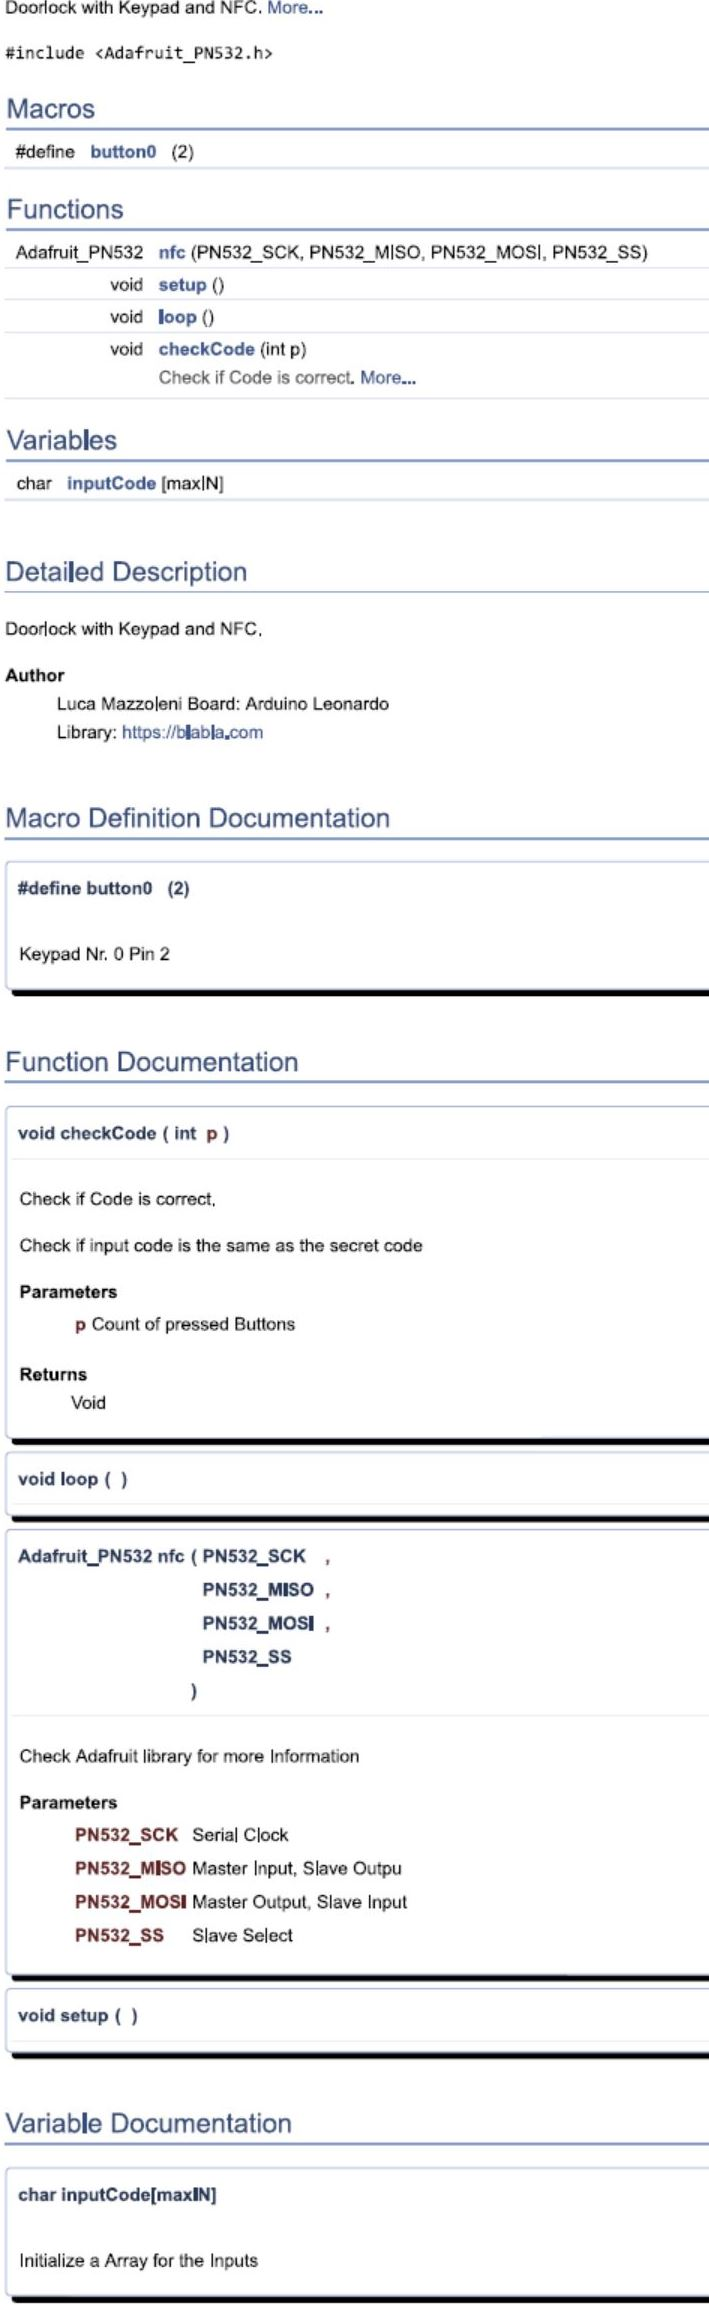
\includegraphics[width=8cm]{images/html.JPG}
\end{multicols}	
\pagebreak
%=================================

\subsection{Qt}
\subsubsection{HTML-Tags}
\lstinputlisting[style=c++qt]{source/Qt/html.cpp}
\begin{longtable}{| p{.15\textwidth} | p{.30\textwidth} | p{.45\textwidth}|}
	\hline \textbf{Tag} & \textbf{Description} & \textbf{Comment}\\
	\hline a& Anchor or link& \\
	\hline address & Address &\\
	\hline b& Bold & \textbf{Fett}\\
	\hline big & Larger font&\\
	\hline blockquote & Indented paragraph&\\
	\hline body & Document body &\\
	\hline br & Line break &\\
	\hline center & Centered paragraph&\\
	\hline cite & Inline citation & Same as i\\
	\hline code & Code& Same as tt\\
	\hline dd & Definition data & \\
	\hline dfn & Definition & \\
	\hline div& Document divison&\\
	\hline em& Emphasized& \emph{Same as i}\\
	\hline font& Font size, family, color& Support size, face, color (Qt::green) attributes\\
	\hline h1 & Level 1 heading& Titel 1. Ordnung\\
	\hline h2 & Level 2 heading& Titel 2. Ordnung\\
	\hline h3 & Level 3 heading& Titel 3. Ordnung\\
	\hline h4 & Level 4 heading& Titel 4. Ordnung\\
	\hline h5 & Level 5 heading& Titel 5. Ordnung\\
	\hline h6 & Level 6 heading& Titel 6. Ordnung\\
	\hline head & Document header&\\
	\hline hr & Horizontal line&\\
	\hline html & HTML document&\\
	\hline i & italic& \textit{kursiv}\\
	\hline img&image& Support src, source, width, height attributes\\
	\hline kbd& User entered text&\\
	\hline meta & Meta-information& Text in Metacode in HTML\\
	\hline li & List-Item& Jeder einzelne Punkt muss umschlossen werden.\\
	\hline nobr & Non-breakable text&\\
	\hline ol & Ordered list& \\
	\hline p & paragraph&\\
	\hline pre & preformated text& \\
	\hline qt & Qt richt-text document& Synonym für HTML\\
	\hline s& Strikethrough&\\
	\hline samp & Sample Code&\\
	\hline small & Small font &{\scriptsize kleine Schrift}\\
	\hline strong & Strong & \textbf{same as b}\\
	\hline style & Style sheet & Allows styling information to be included with rich text\\
	\hline title & Document row & \\
	\hline u & underlined & \\
	\hline var & Variable & Same as i\\
	\hline
\end{longtable}
\clearpage
\newpage
\subsubsection{QWidgets}
\begin{tabular}{c c}
	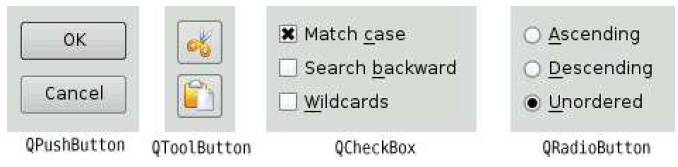
\includegraphics[width=9cm]{images/button_1.png}&
    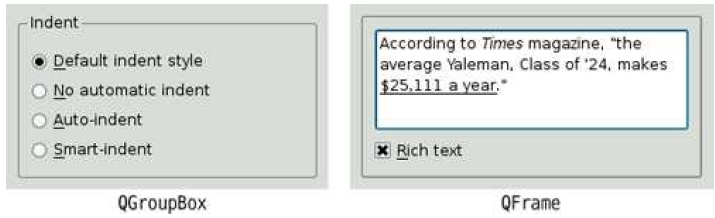
\includegraphics[width=9cm]{images/button_2.png}\\
	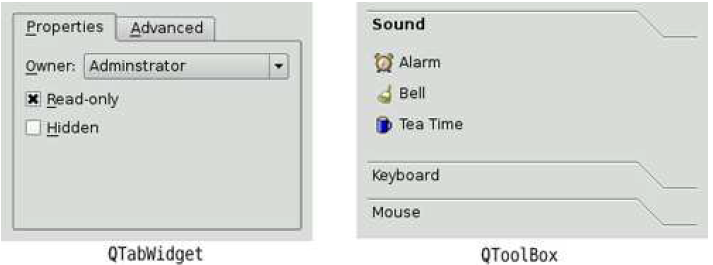
\includegraphics[width=9cm]{images/button_3.png}&
    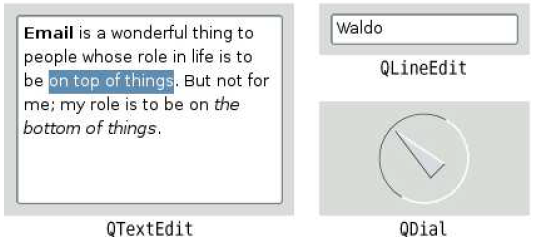
\includegraphics[width=9cm]{images/button_7.png}\\
	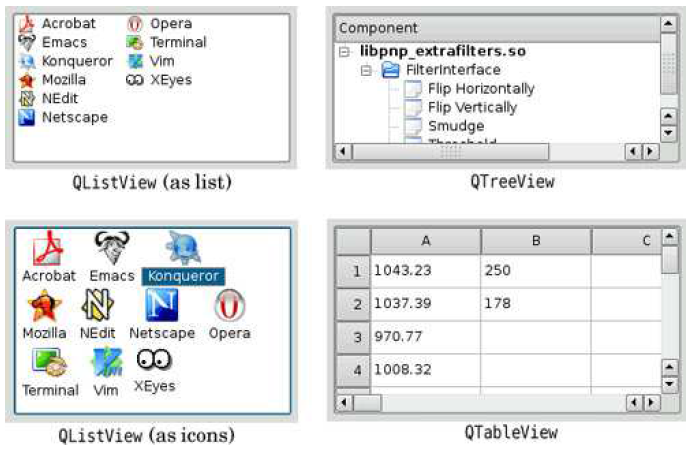
\includegraphics[width=9cm]{images/button_4.png}&
	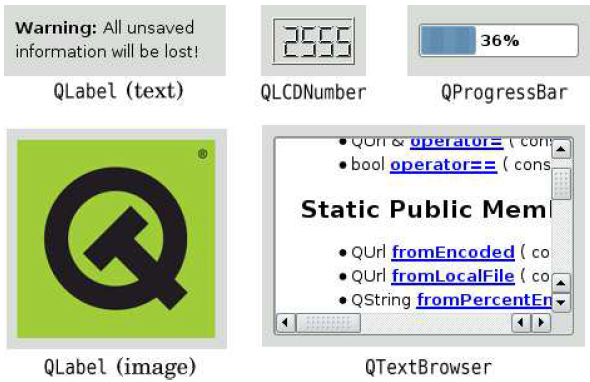
\includegraphics[width=9cm]{images/button_5.png}\\
	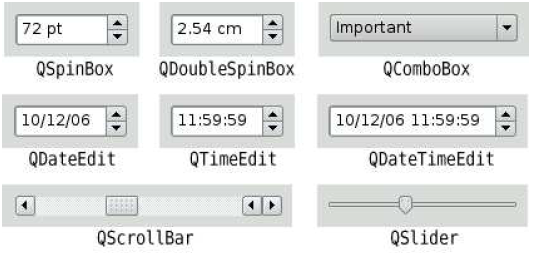
\includegraphics[width=9cm]{images/button_6.png}&
	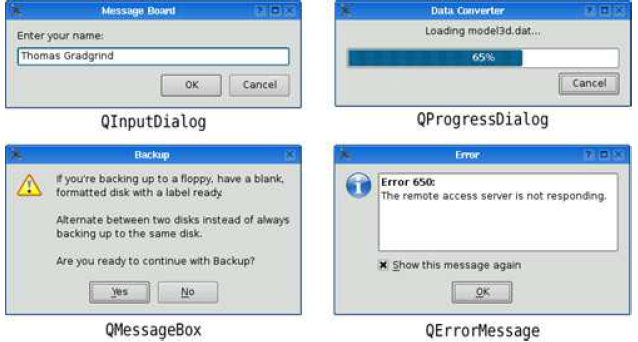
\includegraphics[width=9cm]{images/button_8.png}\\
\end{tabular}
\subsubsection{QBrush}
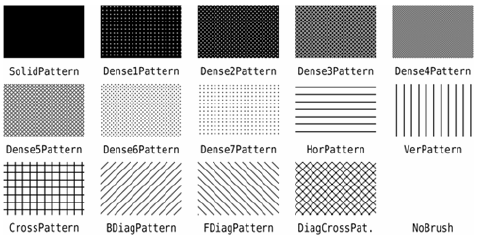
\includegraphics[width=9cm]{images/brush.png}

%\begin{multicols}{2}
    \begin{minipage}{0.6\linewidth}
        \subsubsection{QPainter draw-Methoden}
        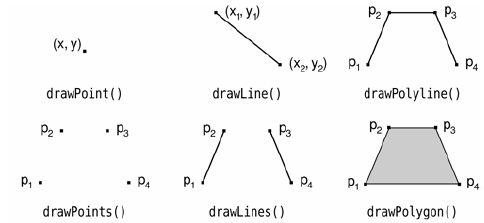
\includegraphics[width=\linewidth]{images/draw_1.png}\newline
        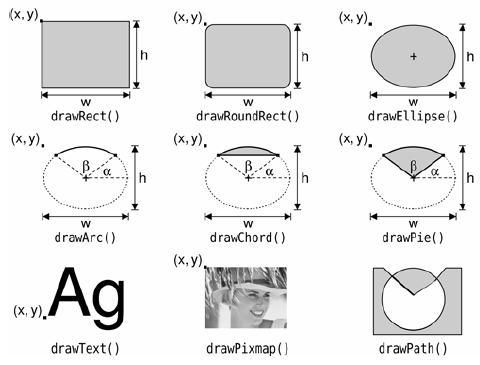
\includegraphics[width=\linewidth]{images/draw_2.png}
    \end{minipage}
    
    \begin{minipage}{0.6\linewidth}
        \subsubsection{QPen}
        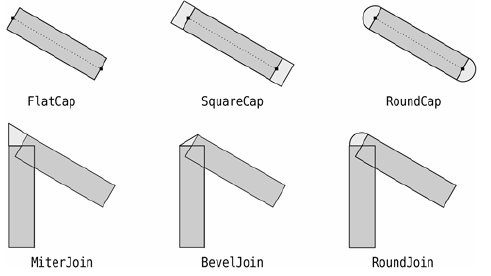
\includegraphics[width=\linewidth]{images/pen_1.png}\newline 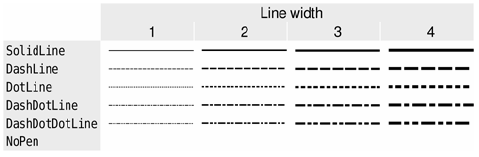
\includegraphics[width=\linewidth]{images/pen_2.png}\newline   
    \end{minipage}
%\end{multicols}
\clearpage
\subsubsection{SpezUeb}
\begin{longtable}{l l} %Error but works.. IDC
    \textbf{GridLayout}&\\
    \lstinputlisting[style=c++qt,linewidth=12cm]{source/Qt/SpezUeb1.cpp}&
    \hspace{-2cm}\includegraphics{images/qtSpezUeb1.jpg}
    \\&\\
    \lstinputlisting[style=c++qt,linewidth=12cm]{source/Qt/GridLayout.cpp}&
    \hspace{-2cm}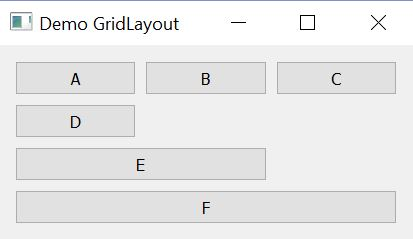
\includegraphics{images/GridLayout.jpg}  
    \\ 
    \\&\\ 
    \textbf{Quiz}&\\
    \lstinputlisting[style=c++qt,linewidth=12cm]{source/Qt/SpezUeb2.cpp}&
    \includegraphics{images/qtSpezUeb2.jpg}
    \\
    \textbf{Signal and Slots}&\\
    \lstinputlisting[style=c++qt,linewidth=12cm]{source/Qt/SpezUeb3.cpp}&
    \hspace{-2cm}\includegraphics{images/qtSpezUeb3.jpg} 
\end{longtable}
%TODO JPG smaller or Print it Standalone A3
%\newpage 
%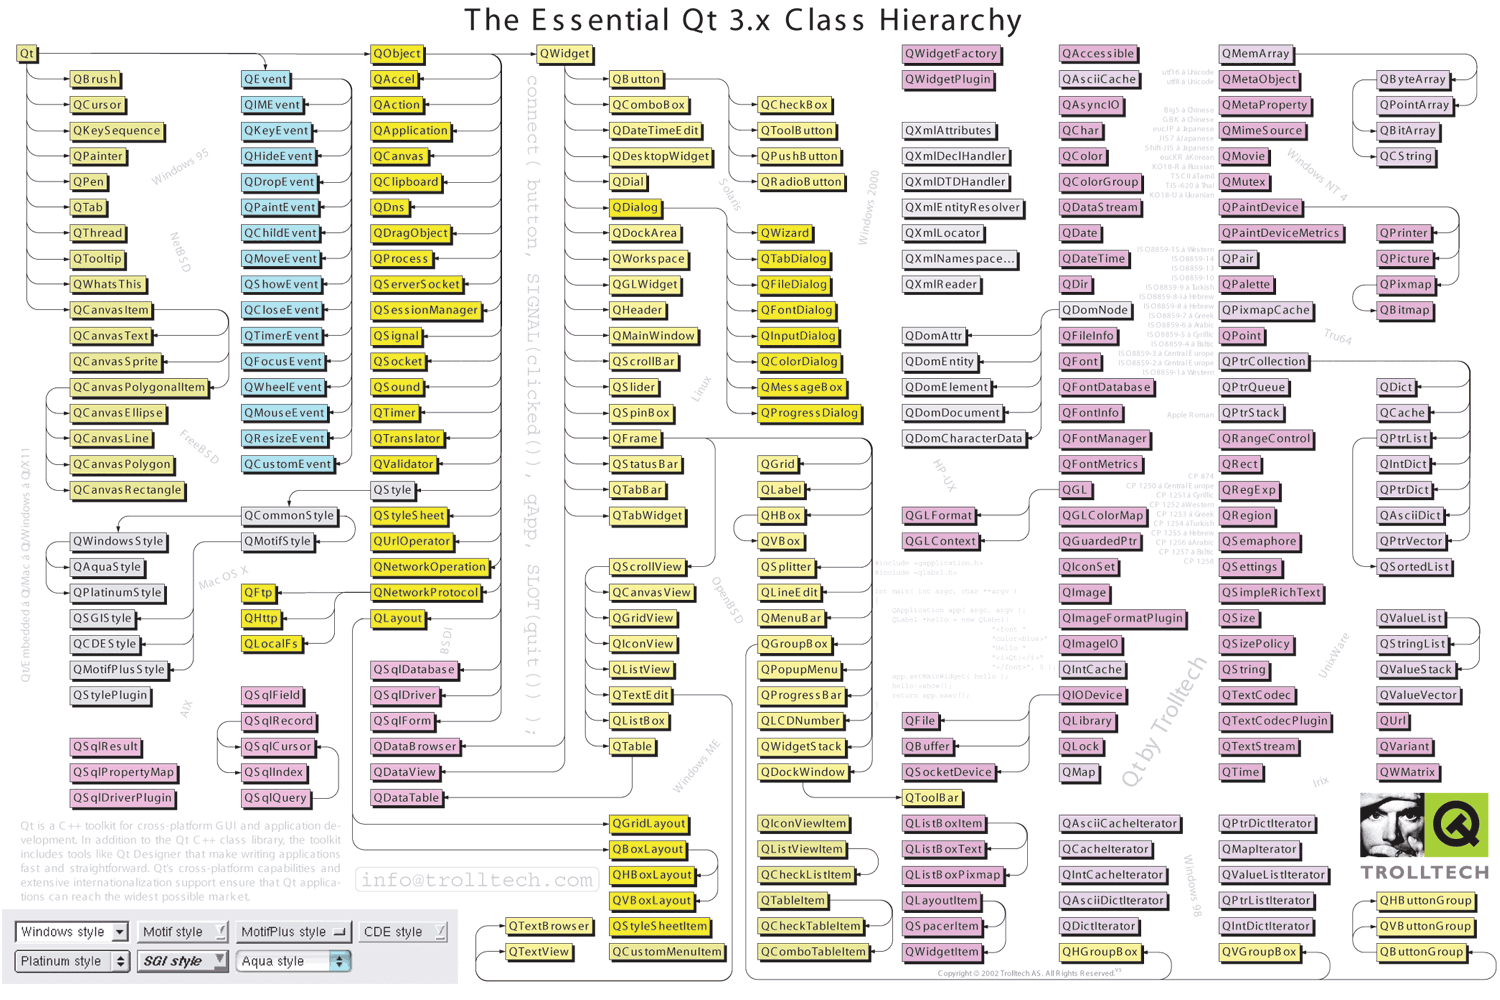
\includegraphics[angle=90,origin=c,width=\linewidth]{images/qt3classchart}
%\newpage
%=================================================
\clearpage
\subsubsection{Hello World}
\lstinputlisting[style=c++qt]{source/Qt/hello_world.cpp}

\subsubsection{Temperaturwidget}
\textbf{main.cpp}
\\
\begin{multicols}{2}
\lstinputlisting[style=c++qt]{source/Qt/main.cpp}

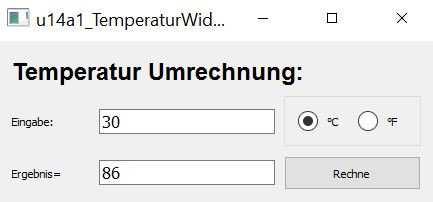
\includegraphics[width=\linewidth]{images/temperaturwidget}
\end{multicols}

\textbf{temperaturwidget.h}
\\
\lstinputlisting[style=c++qt]{source/Qt/temperaturwidget.h}
\newpage
\textbf{temperaturwidget.cpp}
\lstinputlisting[style=c++qt]{source/Qt/temperaturwidget.cpp}

\subsubsection{Counter-implementation}
\begin{multicols}{2}
    \begin{minipage}{\linewidth}
       \textbf{Implementation mit Klassen}\newline
       \textbf{main (Klassen).cpp}
       \lstinputlisting[style=c++qt]{source/Qt/countermain2.cpp}
       \textbf{mydialog.h}
       \lstinputlisting[style=c++qt]{source/Qt/mydialog.h}
       \textbf{mydialog.cpp}
       \lstinputlisting[style=c++qt]{source/Qt/mydialog.cpp}
    \end{minipage}

    \begin{minipage}{\linewidth}
        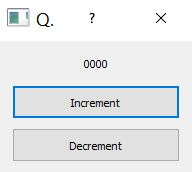
\includegraphics[width=0.5\linewidth]{images/count1}\newline
        \textbf{Implementation \"{}nur\"{} im main.cpp}
        \lstinputlisting[style=c++qt]{source/Qt/countermain1.cpp}
    \end{minipage}
\end{multicols}
\clearpage
\textbf{counter.h}\newline
\lstinputlisting[style=c++qt]{source/Qt/counter.h}
\textbf{counter.cpp}\newline
\lstinputlisting[style=c++qt]{source/Qt/counter.cpp}
%=================================================
\clearpage
\textbf{CircleButton}
\begin{multicols}{2}
    \lstinputlisting[style=c++qt]{source/Qt/CircleButton/main.cpp}
    
\begin{minipage}{0.8\linewidth}
    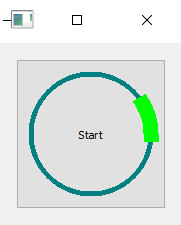
\includegraphics[width=0.5\linewidth]{images/circlebutton1}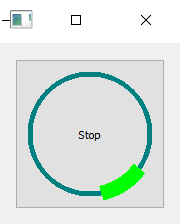
\includegraphics[width=0.5\linewidth]{images/circlebutton2}
    \newline
    \newline
\end{minipage}
\end{multicols}
\lstinputlisting[style=c++qt]{source/Qt/CircleButton/Demo1CircleButton.h}
\lstinputlisting[style=c++qt]{source/Qt/CircleButton/Demo1CircleButton.cpp}
\clearpage
\lstinputlisting[style=c++qt]{source/Qt/CircleButton/CircleButton.h}
\lstinputlisting[style=c++qt]{source/Qt/CircleButton/CircleButton.cpp}



